% Source-faithful schematic draft: 2004 Hunan Arts Q09 options
% Source ID: src-69c1d502b386b3e69e4b98d9f5500c36d4b278d52aa54448a71182edf7c03358
% Source SHA-256: dc0e39533bc2dd37833ae2dc4bdb93e31a39d08808c842611458bf0b844aaeed
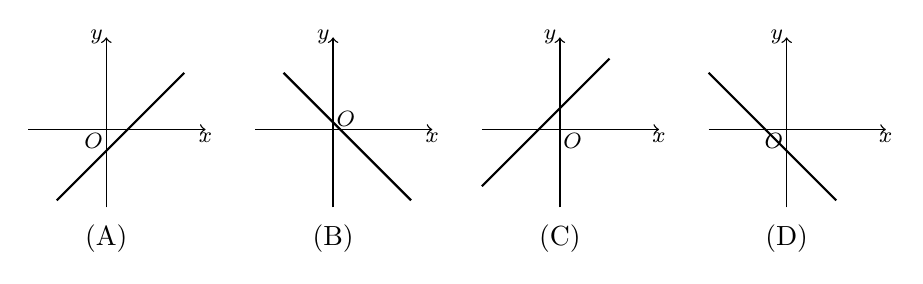
\begin{tikzpicture}[line width=0.5pt,scale=0.9,every node/.style={inner sep=1pt}]
  % Option (A)
  \begin{scope}[xshift=0cm]
    \draw[->] (-1.1,0) -- (1.4,0) node[below] {\footnotesize $x$};
    \draw[->] (0,-1.1) -- (0,1.3) node[left] {\footnotesize $y$};
    \node[below left] at (0,0) {\footnotesize $O$};
    \draw[thick] (-0.7,-1.0) -- (1.1,0.8);
    \node[below] at (0,-1.3) {(A)};
  \end{scope}

  % Option (B)
  \begin{scope}[xshift=3.2cm]
    \draw[->] (-1.1,0) -- (1.4,0) node[below] {\footnotesize $x$};
    \draw[->] (0,-1.1) -- (0,1.3) node[left] {\footnotesize $y$};
    \node[above right] at (0,0) {\footnotesize $O$};
    \draw[thick] (-0.7,0.8) -- (1.1,-1.0);
    \node[below] at (0,-1.3) {(B)};
  \end{scope}

  % Option (C)
  \begin{scope}[xshift=6.4cm]
    \draw[->] (-1.1,0) -- (1.4,0) node[below] {\footnotesize $x$};
    \draw[->] (0,-1.1) -- (0,1.3) node[left] {\footnotesize $y$};
    \node[below right] at (0,0) {\footnotesize $O$};
    \draw[thick] (-1.1,-0.8) -- (0.7,1.0);
    \node[below] at (0,-1.3) {(C)};
  \end{scope}

  % Option (D)
  \begin{scope}[xshift=9.6cm]
    \draw[->] (-1.1,0) -- (1.4,0) node[below] {\footnotesize $x$};
    \draw[->] (0,-1.1) -- (0,1.3) node[left] {\footnotesize $y$};
    \node[below left] at (0,0) {\footnotesize $O$};
    \draw[thick] (-1.1,0.8) -- (0.7,-1.0);
    \node[below] at (0,-1.3) {(D)};
  \end{scope}
\end{tikzpicture}
